%%%%%%%%%%%%%%%%%%%%%%%%%%%%%%%%%%%%%%%%%
% University Assignment Title Page 
% LaTeX Template
% Version 1.0 (27/12/12)
%
% This template has been downloaded from:
% http://www.LaTeXTemplates.com
%
% Original author:
% WikiBooks (http://en.wikibooks.org/wiki/LaTeX/Title_Creation)
%
% License:
% CC BY-NC-SA 3.0 (http://creativecommons.org/licenses/by-nc-sa/3.0/)
% 
% Instructions for using this template:
% This title page is capable of being compiled as is. This is not useful for 
% including it in another document. To do this, you have two options: 
%
% 1) Copy/paste everything between \begin{document} and \end{document} 
% starting at \begin{titlepage} and paste this into another LaTeX file where you 
% want your title page.
% OR
% 2) Remove everything outside the \begin{titlepage} and \end{titlepage} and 
% move this file to the same directory as the LaTeX file you wish to add it to. 
% Then add \input{./title_page_1.tex} to your LaTeX file where you want your
% title page.
%
%%%%%%%%%%%%%%%%%%%%%%%%%%%%%%%%%%%%%%%%%
%\title{Title page with logo}
%----------------------------------------------------------------------------------------
%	PACKAGES AND OTHER DOCUMENT CONFIGURATIONS
%----------------------------------------------------------------------------------------

\documentclass[12pt]{article}
\usepackage[utf8]{inputenc}
\usepackage[MeX]{polski}
\usepackage{amsmath}
\usepackage{graphicx}
\usepackage{listings}
\usepackage{color}
\usepackage{indentfirst}

% Kolory
\definecolor{dkgreen}{rgb}{0,0.6,0}
\definecolor{gray}{rgb}{0.5,0.5,0.5}
\definecolor{mauve}{rgb}{0.58,0,0.82}

% Mniejsze marginesy
\addtolength{\textwidth}{3cm}
\addtolength{\hoffset}{-1.5cm}
\addtolength{\textheight}{3cm}
\addtolength{\voffset}{-1.5cm}

% SQLite
\lstdefinestyle{SQLite}{
	frame=tb,
	language=SQL,
	aboveskip=3mm,
	belowskip=3mm,
	showstringspaces=false,
	columns=flexible,
	basicstyle={\small\ttfamily},
	numbers=none,
	numberstyle=\tiny\color{gray},
	keywordstyle=\color{blue},
	commentstyle=\color{dkgreen},
	stringstyle=\color{mauve},
	breaklines=true,
	breakatwhitespace=true,
	tabsize=3,
	keywords={TEXT},
	emphstyle=\color{blue},
}

% Java
\lstdefinestyle{Java}{
	frame=tb,
	language=Java,
	aboveskip=3mm,
	belowskip=3mm,
	showstringspaces=false,
	columns=flexible,
	basicstyle={\small\ttfamily},
	numbers=none,
	numberstyle=\tiny\color{gray},
	keywordstyle=\color{blue},
	commentstyle=\color{dkgreen},
	stringstyle=\color{mauve},
	breaklines=true,
	breakatwhitespace=true,
	tabsize=3,
}

% Kod
\lstset{
	frame=tb,
	aboveskip=3mm,
	belowskip=3mm,
	showstringspaces=false,
	columns=flexible,
	basicstyle={\small\ttfamily},
	numbers=none,
	breaklines=true,
	breakatwhitespace=true,
	tabsize=3,
}

% Odstęp po akapicie
\setlength{\parskip}{1ex plus 0.5ex minus 0.5ex}

\begin{document}

\begin{titlepage}

\newcommand{\HRule}{\rule{\linewidth}{0.5mm}} % Defines a new command for the horizontal lines, change thickness here

\center % Center everything on the page
 
%----------------------------------------------------------------------------------------
%	HEADING SECTIONS
%----------------------------------------------------------------------------------------

\textsc{\large Politechnika Wrocławska}\\[4cm] % Name of your university/college
\textsc{\Large Bazy danych 2}\\[0.5cm] % Major heading such as course name
\textsc{\large projekt}\\[0.5cm] % Minor heading such as course title

%----------------------------------------------------------------------------------------
%	TITLE SECTION
%----------------------------------------------------------------------------------------

\HRule \\[0.6cm]
{\huge \bfseries Dokumentacja projektu}\\[0.4cm] % Title of your document
\textsc{\Large Stacjonarny sklep muzyczny}\\[0.4cm]
\HRule \\[0.5cm]
 
%----------------------------------------------------------------------------------------
%	AUTHOR SECTION
%----------------------------------------------------------------------------------------

{\textsc{\large termin zajęć: poniedziałek 13:15}}\\[1.0cm]

\begin{minipage}{0.4\textwidth}
	\begin{flushleft} \large
		\emph{Autorzy:}\\[0.1cm]
		Jakub \textsc{Białecki}, 218281
		\newline
		Damian \textsc{Korzekwa}, 226132
	\end{flushleft}
\end{minipage}
~
\begin{minipage}{0.5\textwidth}
	\begin{flushright} \large
		\emph{Prowadzący:} \\[0.1cm]
		dr inż. Roman \textsc{Ptak}
	\end{flushright}
\end{minipage}\\[1cm]

% If you don't want a supervisor, uncomment the two lines below and remove the section above
%\Large \emph{Author:}\\
%John \textsc{Smith}\\[3cm] % Your name

%----------------------------------------------------------------------------------------
%	DATE SECTION
%----------------------------------------------------------------------------------------

%{\large \today}\\[2cm] % Date, change the \today to a set date if you want to be precise

%----------------------------------------------------------------------------------------
%	LOGO SECTION
%----------------------------------------------------------------------------------------

%\includegraphics{logo.png}\\[1cm] % Include a department/university logo - this will require the graphicx package
 
%----------------------------------------------------------------------------------------

\vfill % Fill the rest of the page with whitespace

{\large Wrocław 2018}

\end{titlepage}

%%%%%%%%%%%%%%%%%%%%%%%%%%%%%%%%%%%%%%%%%%%%%%%%%%%%%%%%%%%%%%%%
\section{Wstęp}
%%%%%%%%%%%%%%%%%%%%%%%%%%%%%%%%%%%%%%%%%%%%%%%%%%%%%%%%%%%%%%%%
%%%%%%%%%%%%%%%%%%%%%%%%%%%%%%%%%%%%%%%%%%%%%%%%
\subsection{Cel projektu}
%%%%%%%%%%%%%%%%%%%%%%%%%%%%%%%%%%%%%%%%%%%%%%%%

Celem projektu było stworzenie bazy danych wraz z aplikacją dostępową dla stacjonarnego sklepu muzycznego.

%%%%%%%%%%%%%%%%%%%%%%%%%%%%%%%%%%%%%%%%%%%%%%%%
\subsection{Zakres projektu}
%%%%%%%%%%%%%%%%%%%%%%%%%%%%%%%%%%%%%%%%%%%%%%%%

Utworzona w projekcie baza danych zawiera informacje o produktach, które są sprzedawane w sklepie.

Dodatkowo, baza danych ma za zadanie przechowywać historię transakcji - zarówno transakcje sprzedaży towaru klientom, jak i zamówienia przez sklep produktów z zewnętrznych magazynów.

Aplikacja dostępowa ma umożliwiać właścicielowi i pracownikom sklepu dostęp do tej bazy - łatwe dodawanie nowych produktów, edycję już istniejących, usuwanie produktów oraz przeglądanie historii transakcji.

%%%%%%%%%%%%%%%%%%%%%%%%%%%%%%%%%%%%%%%%%%%%%%%%%%%%%%%%%%%%%%%%
\section{Analiza wymagań} \label{analiza_wymagan}
%%%%%%%%%%%%%%%%%%%%%%%%%%%%%%%%%%%%%%%%%%%%%%%%%%%%%%%%%%%%%%%%
%%%%%%%%%%%%%%%%%%%%%%%%%%%%%%%%%%%%%%%%%%%%%%%%
\subsection{Opis działania i schemat logiczny systemu}
%%%%%%%%%%%%%%%%%%%%%%%%%%%%%%%%%%%%%%%%%%%%%%%%

Sklep muzyczny „Guitar Hero” znajduje się we Wrocławiu przy ulicy Ruskiej 11. Sklep zajmuje się sprzedażą instrumentów muzycznych. Dodatkowo, w ofercie sklepu, znajdują się artykuły okołomuzyczne.

Sklep prowadzony jest przez właściciela i to on decyduje o tym, jaki asortyment znajduje się w sklepie. Ponadto sklep zatrudnia pracowników, którzy zajmują się doradzaniem klientom sklepu, obsługą zamówień, sprzedażą oraz zarządzaniem towarem w sklepie.

W związku z tym, że lokal nie jest duży, sklep posiada magazyn, w którym przechowywane są instrumenty. W sklepie wystawiona jest jedynie część towaru. Magazyn znajduje się około 500 metrów od sklepu. Towar może być dostarczony z magazynu do sklepu na prośbę klienta lub klient może odebrać towar z magazynu za okazaniem paragonu lub faktury.

Aplikacja wraz z bazą danych ma za zadanie ułatwić właścicielowi, jak i pracownikom sklepu, zarządzanie oferowanymi produktami oraz historią transakcji.

%%%%%%%%%%%%%%%%%%%%%%%%%%%%%%%%%%%%%%%%%%%%%%%%
\subsection{Wymagania funkcjonalne}
%%%%%%%%%%%%%%%%%%%%%%%%%%%%%%%%%%%%%%%%%%%%%%%%

\begin{itemize}
	\item właściciel sklepu ma możliwość dodawania nowych produktów do bazy danych
	
	\item właściciel sklepu ma możliwość pełnej modyfikacji dodanych produktów w bazie danych
	
	\item właściciel ma możliwość usuwania (wycofania z oferty) produktów z bazy danych
	
	\item właściciel ma możliwość dodawania nowych kategorii produktów
	
	\item zarówno pracownik jak i właściciel mogą przeglądać historię transakcji
	
	\item właściciel i pracownik mają możliwość sprzedaży produktu klientowi (usunięcia egzemplarza produktu z bazy danych) i tym samym dodania takiej transakcji do historii
	
	\item właściciel i pracownik mają możliwość zamówienia kolejnych egzemplarzy produktów (dodania nowego egzemplarza produktu do bazy danych) i tym samym dodania takiej transakcji do historii
\end{itemize}

%%%%%%%%%%%%%%%%%%%%%%%%%%%%%%%%%%%%%%%%%%%%%%%%
\subsection{Wymagania niefunkcjonalne}
%%%%%%%%%%%%%%%%%%%%%%%%%%%%%%%%%%%%%%%%%%%%%%%%

\begin{itemize}
	\item baza danych będzie przechowywać informacje o produktach oferowanych w sklepie wraz ze szczegółowymi informacjami na temat produktu (id, nazwa produktu, cena katalogowa, cena promocyjna, stan magazynowy, stan produktu (nowy, używany, powystawowy), kategoria, opis)
	
	\item baza danych będzie przechowywać również historię transakcji wraz ze szczegółowymi informacjami (id transakcji, kwota, strona transakcji (klient-sklep, sklep-producent), data transakcji, produkt transakcji, ilość produktów)
\end{itemize}

%%%%%%%%%%%%%%%%%%%%%%%%%%%%%%%%
\subsubsection{Wykorzystywane technologie i narzędzia}
%%%%%%%%%%%%%%%%%%%%%%%%%%%%%%%%

Baza danych będzie wykorzystywać technologię SQLite. Aplikacja dostępowa będzie napisana w języku Java z interfejsem graficznym wykorzystującym technologię JavaFX. Dostęp do bazy danych z poziomu aplikacji w Javie planujemy zapewnić przy użyciu biblioteki JDBC lub SQLJet.

Planujemy wykorzystać IntelliJ IDEA Community jako główne środowisko programistyczne oraz Gita jako system kontroli wersji.

%%%%%%%%%%%%%%%%%%%%%%%%%%%%%%%%
\subsubsection{Wymagania dotyczące rozmiaru bazy danych}
%%%%%%%%%%%%%%%%%%%%%%%%%%%%%%%%

Szacujemy, że w sklepie będzie w sprzedaży około kilka/kilkanaście tysięcy produktów. Nie wszystkie będą dostępne od razu w sklepie, jednak baza danych musi przechowywać o nich informacje.

Zakładamy, że sklep będzie realizował średnio 15 - 30 transakcji dziennie. Szacujemy ilość transakcji w takiej bazie na około 60000 po około pięciu latach funkcjonowania sklepu.

%%%%%%%%%%%%%%%%%%%%%%%%%%%%%%%%
\subsubsection{Wymagania dotyczące bezpieczeństwa systemu}
%%%%%%%%%%%%%%%%%%%%%%%%%%%%%%%%

Z racji tego, iż sklep prowadzi jedynie sprzedaż stacjonarną, baza danych nie wymaga specjalistycznych zabezpieczeń. Podstawowym zabezpieczeniem bazy będzie system logowania dla pracowników (w tym dla właściciela sklepu).

%%%%%%%%%%%%%%%%%%%%%%%%%%%%%%%%%%%%%%%%%%%%%%%%
\subsection{Przyjęte założenia projektowe}
%%%%%%%%%%%%%%%%%%%%%%%%%%%%%%%%%%%%%%%%%%%%%%%%

\begin{itemize}
	
	\item relacje pomiędzy kluczami głównymi a obcymi
	
	\item odpowiednie typy danych i ich wielkości
	
	\item użyć odpowiedniego nazewnictwa tabel, kluczy głównych i kluczy obcych
	
	\item utworzenie widoków, zwracające istotne dane w sensie działania aplikacji
	
	\item użycie złączeń
	
	\item utworzenie funkcji dokonujących na danych w tabelach takich operacji jak: dodawanie, usuwanie i aktualizacja
	
\end{itemize}

\newpage
%%%%%%%%%%%%%%%%%%%%%%%%%%%%%%%%%%%%%%%%%%%%%%%%%%%%%%%%%%%%%%%%
\section{Projekt systemu}
%%%%%%%%%%%%%%%%%%%%%%%%%%%%%%%%%%%%%%%%%%%%%%%%%%%%%%%%%%%%%%%%
%%%%%%%%%%%%%%%%%%%%%%%%%%%%%%%%%%%%%%%%%%%%%%%%
\subsection{Projekt bazy danych}
%%%%%%%%%%%%%%%%%%%%%%%%%%%%%%%%%%%%%%%%%%%%%%%%
%%%%%%%%%%%%%%%%%%%%%%%%%%%%%%%%
\subsubsection{Analiza rzeczywistości i uproszczony model konceptualny}
%%%%%%%%%%%%%%%%%%%%%%%%%%%%%%%%

Na podstawie analizy przedstawionej w rozdziale \ref{analiza_wymagan}, stworzyliśmy konceptualny bazy danych dla sklepu, który został przedstawiony na rysunku \ref{image1}.

\begin{figure}[h]
	\centering
	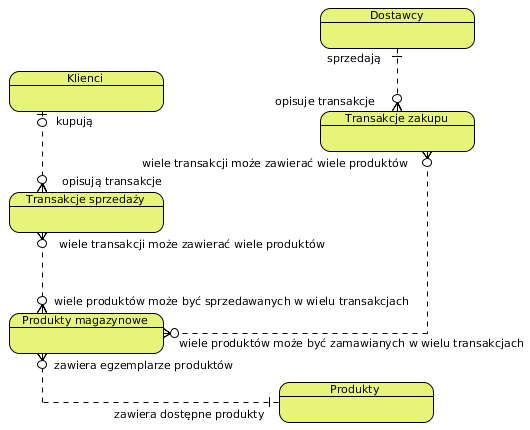
\includegraphics[width=0.8\linewidth]{images/image1.png}
	\caption{Model konceptualny}
	\label{image1}
\end{figure}

\newpage
%%%%%%%%%%%%%%%%%%%%%%%%%%%%%%%%
\subsubsection{Model logiczny i normalizacja}
%%%%%%%%%%%%%%%%%%%%%%%%%%%%%%%%

Następnym krokiem było rozbudowanie modelu konceptualnego o nowe tabele, uzupełnienie tabel o kolumny oraz zdefiniowanie bardziej szczegółowych relacji między tabelami. Rysunek \ref{image2} przedstawia gotowy model logiczny.

\begin{figure}[h]
	\centering
	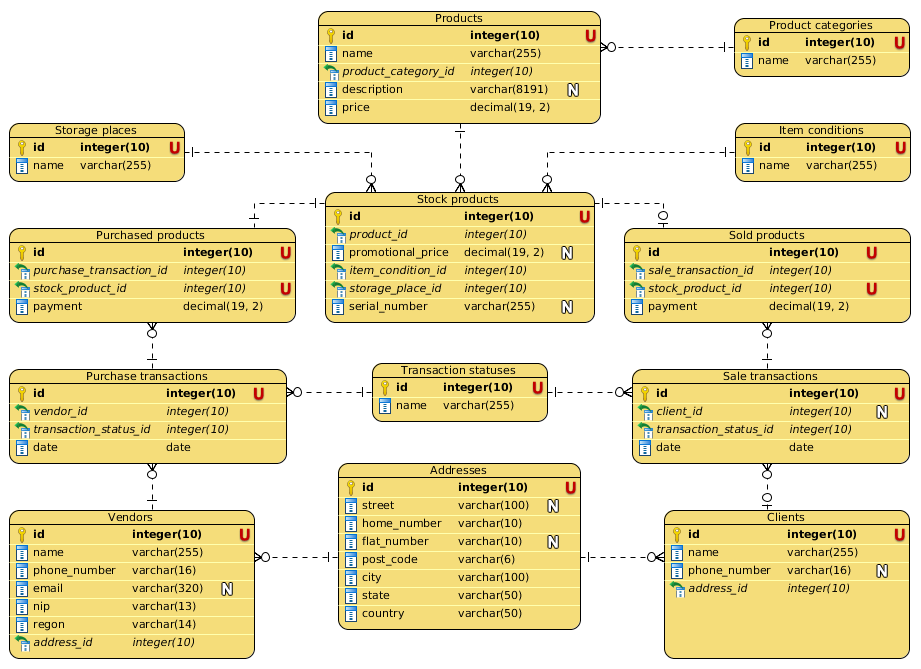
\includegraphics[width=1\linewidth]{images/image2.png}
	\caption{Model logiczny}
	\label{image2}
\end{figure}

\newpage
%%%%%%%%%%%%%%%%%%%%%%%%%%%%%%%%
\subsubsection{Model fizyczny i ograniczenia integralności danych}
%%%%%%%%%%%%%%%%%%%%%%%%%%%%%%%%

Po stworzeniu modelu logicznego, przeszliśmy do stworzenia modelu fizycznego bazy danych. Po głębszej analizie, okazało się, że w SQLite nie ma możliwości wprowadzenia ograniczeń wielkości danych w poszczególnych kolumnach. Dodatkowo, ustalone przez nas wstępnie typy danych należało zmienić na zdecydowanie bardziej uproszczone. Rysunek \ref{image3} przedstawia gotowy model.

\begin{figure}[h]
	\centering
	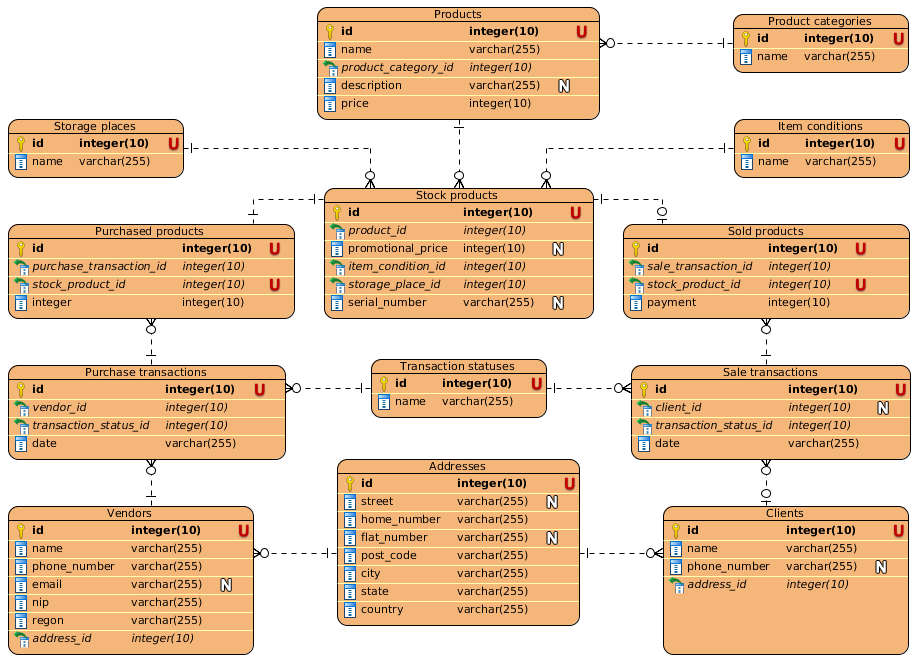
\includegraphics[width=1\linewidth]{images/image3.png}
	\caption{Model logiczny}
	\label{image3}
\end{figure}

Wszystkie możliwe typy danych sprowadziliśmy do dwóch: \lstinline[style=SQLite]|varchar(255)| oraz \lstinline[style=SQLite]|integer(10)|. Z powodu ograniczeń programu Visual Paradigm nie byliśmy w stanie zamienić tych typów na te, które rzeczywiście występują w SQLite, czyli odpowiednio \lstinline[style=SQLite]|TEXT| oraz \lstinline[style=SQLite]|INTEGER|.

%%%%%%%%%%%%%%%%%%%%%%%%%%%%%%%%
\subsubsection{Inne elementy schematu – mechanizmy przetwarzania danych}
%%%%%%%%%%%%%%%%%%%%%%%%%%%%%%%%

\begin{itemize}
	
	\item \textbf{Indeksy}
	
	Celem indeksów jest przyspieszenie operacji wyszukiwania, więc starano się znaleźć atrybuty, po których pracownik będzie najczęściej przeszukiwał tabelę. Oczywiście indeksy mają swoje wady. Wydłużają one czas wykonywania operacji wstawiania, modyfikacji i~usuwania w tabeli.
	
	Zdecydowaliśmy się na stworzenie następujących indeksów:
	
	\begin{itemize}
		
		\item \lstinline|stock_products_index| – \lstinline|product_id|, \lstinline|storage_place_id|, \lstinline|serial_number|
		
		\item \lstinline|clients_index| – \lstinline|name|, \lstinline|phone_number|, \lstinline|address_id|
		
		\item \lstinline|vendors_index| – \lstinline|name|, \lstinline|address_id|, \lstinline|phone_number|
		
	\end{itemize}
	
	\item \textbf{Widoki}
	
	Widoki umożliwiają dostęp do podzbioru kolumn i wierszy tabel lub tabeli.
	
	Gdy korzysta się często z jakiejś tabeli ze stałymi parametrami warto stworzyć widok, w celu zaoszczędzenia czasu. Widoku używa się także gdy jest potrzeba ograniczenia dostępu użytkownika.
	
	Zdecydowaliśmy się na zdefiniowanie następujących widoków:
	
	\begin{itemize}
		
		\item  z ograniczeniem \lstinline|WITH READ ONLY| tabeli \lstinline|products| i \lstinline|product_categories| do której dostęp będą mieli pracownicy bez uprawnień właściciela
		
	\end{itemize}
	
\end{itemize}

%%%%%%%%%%%%%%%%%%%%%%%%%%%%%%%%
\subsubsection{Projekt mechanizmów bezpieczeństwa na poziomie bazy danych}
%%%%%%%%%%%%%%%%%%%%%%%%%%%%%%%%

\begin{itemize}
	
	\item \textbf{Kopie zapasowe}
	
	Dane w bazie danych są archiwizowane raz na pół roku. Okresowo kopie zapasowe powinny być testowane pod względem rzeczywistej możliwości wykorzystania ich w sytuacji koniecznej. Dane dotyczące płatności są przechowywane przez 5 lat. Dane o klientach i~zamówieniach są przechowywane przez 5 lat.
	
	\newpage
	\item \textbf{Uprawnienia użytkowników}
	
	W - uprawnienia właściciela sklepu
	
	P - uprawnienia pracownika
	
\end{itemize}

\begin{table}[h]
	\centering
	\caption{Uprawnienia użytkowników}
	\label{my-label}
	\begin{tabular}{lllll}
		\hline
		Tabela & Dodawanie & Modyfikacja & Usuwanie & Przeglądanie \\ \hline
		addresses & W, P & W & W & W \\
		clients & W, P & W & W & W \\
		item\_conditions & W & W & W & W, P \\
		product\_categories & W & W & W & W, P \\
		products & W & W & W & W, P \\
		purchase\_transactions & W, P & W & W & W, P \\
		purchased\_products & W, P & W & W & W, P \\
		sale\_transactions& W, P & W & W & W, P \\
		sold\_products& W, P & W & W & W, P \\
		stock\_products& W, P & W, P & W, P & W, P \\
		storage\_places& W & W & W & W, P \\
		transaction\_statuses& W & W & W & W \\
		vendors & W, P & W & W & W \\ \hline
	\end{tabular}
\end{table}

\newpage
%%%%%%%%%%%%%%%%%%%%%%%%%%%%%%%%%%%%%%%%%%%%%%%%
\subsection{Projekt aplikacji użytkownika}
%%%%%%%%%%%%%%%%%%%%%%%%%%%%%%%%%%%%%%%%%%%%%%%%
%%%%%%%%%%%%%%%%%%%%%%%%%%%%%%%%
\subsubsection{Architektura aplikacji i diagramy projektowe}
%%%%%%%%%%%%%%%%%%%%%%%%%%%%%%%%

Utworzyliśmy następujący diagram przypadków użycia aplikacji, widoczny na rysunku \ref{image4}.

\begin{figure}[h]
	\centering
	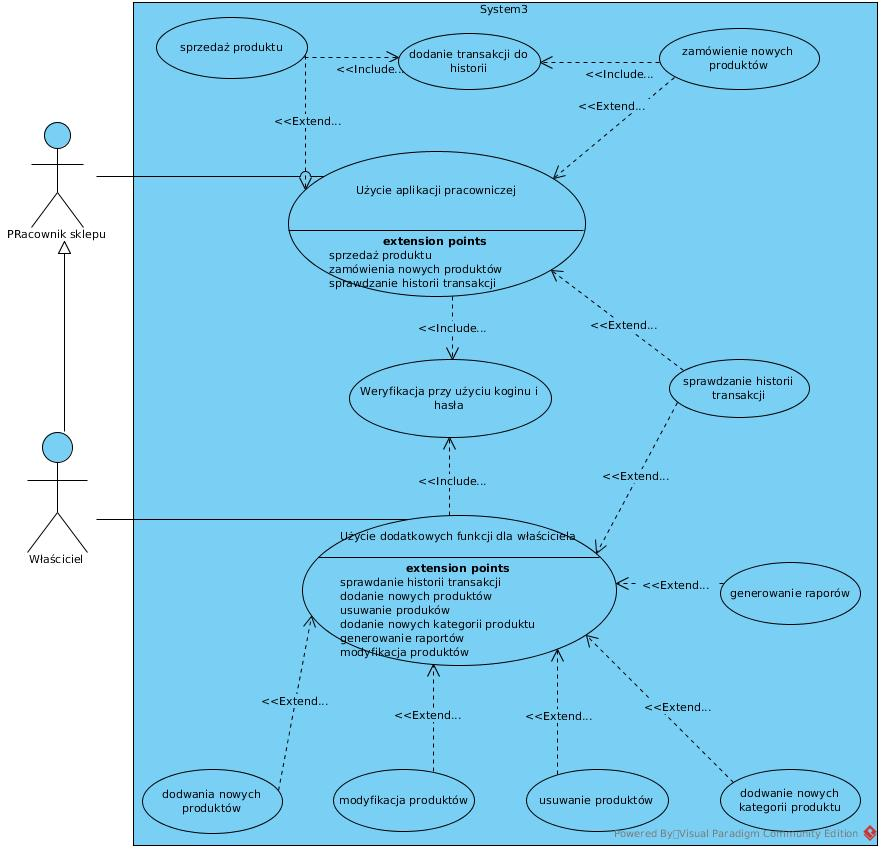
\includegraphics[width=0.8\linewidth]{images/image4.jpg}
	\caption{Diagram przypadków użycia}
	\label{image4}
\end{figure}

\newpage
%%%%%%%%%%%%%%%%%%%%%%%%%%%%%%%%
\subsubsection{Interfejs graficzny i struktura menu}
%%%%%%%%%%%%%%%%%%%%%%%%%%%%%%%%

Wstępny projekt interfejsu wykonaliśmy w programie Pencil. Efekty można zobaczyć na~rysunkach \ref{image5} i \ref{image6}.

\begin{figure}[h]
	\centering
	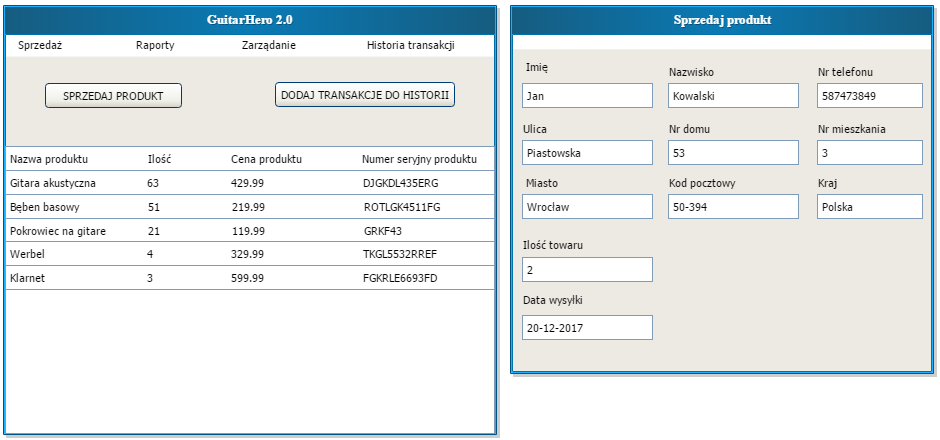
\includegraphics[width=0.8\linewidth]{images/image5.png}
	\caption{Projekt interfejsu graficznego}
	\label{image5}
\end{figure}

\begin{figure}[h]
	\centering
	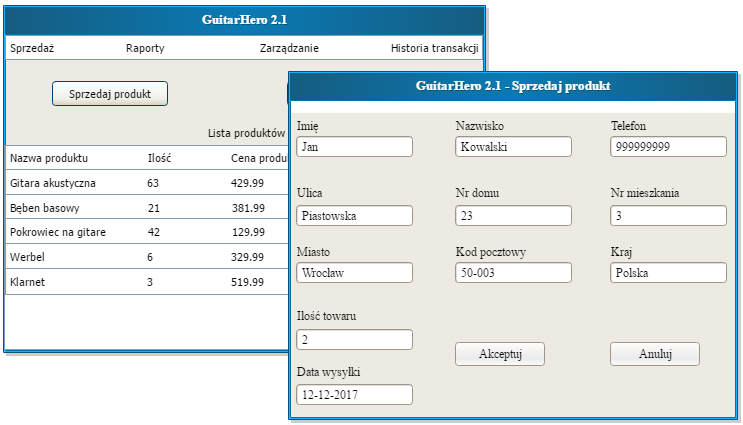
\includegraphics[width=0.8\linewidth]{images/image6.png}
	\caption{Projekt interfejsu graficznego}
	\label{image6}
\end{figure}

\newpage
%%%%%%%%%%%%%%%%%%%%%%%%%%%%%%%%
\subsubsection{Projekt wybranych funkcji systemu}
%%%%%%%%%%%%%%%%%%%%%%%%%%%%%%%%

\begin{figure}[h]
	\centering
	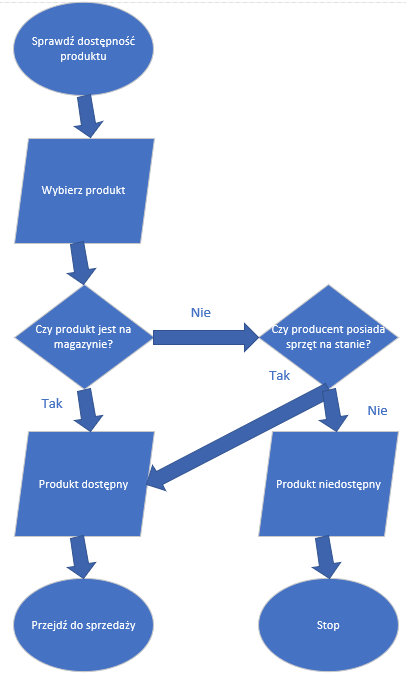
\includegraphics[width=0.5\linewidth]{images/image11.png}
	\caption{Projekt funkcji systemu}
	\label{image11}
\end{figure}

%%%%%%%%%%%%%%%%%%%%%%%%%%%%%%%%
\subsubsection{Metoda podłączania do bazy danych – integracja z bazą danych}
%%%%%%%%%%%%%%%%%%%%%%%%%%%%%%%%

Jako bazę danych dla aplikacji wybraliśmy SQLite, ponieważ jest to lekka baza i w pełni wystarczająca do obsługi sklepu.

Dostęp do bazy będziemy zapewniać przy użyciu JDBC w Javie.

%%%%%%%%%%%%%%%%%%%%%%%%%%%%%%%%
\subsubsection{Projekt zabezpieczeń na poziomie aplikacji}
%%%%%%%%%%%%%%%%%%%%%%%%%%%%%%%%

Aplikacja zapewniać będzie zabezpieczenia do bazy danych za pomocą loginu i hasła podawanego w aplikacji.

%%%%%%%%%%%%%%%%%%%%%%%%%%%%%%%%%%%%%%%%%%%%%%%%%%%%%%%%%%%%%%%%
\section{Implementacja systemu baz danych}
%%%%%%%%%%%%%%%%%%%%%%%%%%%%%%%%%%%%%%%%%%%%%%%%%%%%%%%%%%%%%%%%
%%%%%%%%%%%%%%%%%%%%%%%%%%%%%%%%%%%%%%%%%%%%%%%%
\subsection{Tworzenie tabel i definiowanie ograniczeń}
%%%%%%%%%%%%%%%%%%%%%%%%%%%%%%%%%%%%%%%%%%%%%%%%

Do stworzenia tabel wykorzystaliśmy program DB Browser, który zapewnił możliwość stworzenia praktycznie całej bazy danych bez znajomości języka SQL. Kod dla poszczególnych tabel wygenerowanych przez program prezentujemy poniżej.

Tabela \lstinline|addresses|:

\begin{lstlisting}[style=SQLite]
CREATE TABLE `addresses` (
	`id`	INTEGER NOT NULL PRIMARY KEY AUTOINCREMENT UNIQUE,
	`street`	TEXT,
	`home_number`	TEXT NOT NULL,
	`flat_number`	TEXT,
	`post_code`	TEXT NOT NULL,
	`city`	TEXT NOT NULL,
	`state`	TEXT NOT NULL,
	`country`	TEXT NOT NULL
);
\end{lstlisting}

Tabela \lstinline|clients|:

\begin{lstlisting}[style=SQLite]
CREATE TABLE `clients` (
	`id`	INTEGER NOT NULL PRIMARY KEY AUTOINCREMENT UNIQUE,
	`name`	TEXT NOT NULL,
	`phone_number`	TEXT,
	`address_id`	INTEGER NOT NULL,
	FOREIGN KEY(`address_id`) REFERENCES `addresses`(`id`)
);
\end{lstlisting}

Tabela \lstinline|item_conditions|:

\begin{lstlisting}[style=SQLite]
CREATE TABLE `item_conditions` (
	`id`	INTEGER NOT NULL PRIMARY KEY AUTOINCREMENT UNIQUE,
	`name`	TEXT NOT NULL
);
\end{lstlisting}

Tabela \lstinline|product_categories|:

\begin{lstlisting}[style=SQLite]
CREATE TABLE `product_categories` (
	`id`	INTEGER NOT NULL PRIMARY KEY AUTOINCREMENT UNIQUE,
	`name`	TEXT NOT NULL
);
\end{lstlisting}

Tabela \lstinline|products|:

\begin{lstlisting}[style=SQLite]
CREATE TABLE `products` (
	`id`	INTEGER NOT NULL PRIMARY KEY AUTOINCREMENT UNIQUE,
	`name`	TEXT NOT NULL,
	`product_category_id`	INTEGER NOT NULL,
	`description`	TEXT,
	`price`	INTEGER NOT NULL,
	FOREIGN KEY(`product_category_id`) REFERENCES `product_categories`(`id`)
);
\end{lstlisting}

Tabela \lstinline|purchase_transactions|:

\begin{lstlisting}[style=SQLite]
CREATE TABLE `purchase_transactions` (
	`id`	INTEGER NOT NULL PRIMARY KEY AUTOINCREMENT UNIQUE,
	`vendor_id`	INTEGER NOT NULL,
	`transaction_status_id`	INTEGER NOT NULL,
	`date`	TEXT NOT NULL,
	FOREIGN KEY(`transaction_status_id`) REFERENCES `transaction_statuses`(`id`),
	FOREIGN KEY(`vendor_id`) REFERENCES `vendors`(`id`)
);
\end{lstlisting}

Tabela \lstinline|purchased_products|:

\begin{lstlisting}[style=SQLite]
CREATE TABLE `purchased_products` (
	`id`	INTEGER NOT NULL PRIMARY KEY AUTOINCREMENT UNIQUE,
	`purchase_transaction_id`	INTEGER NOT NULL,
	`stock_product_id`	INTEGER NOT NULL UNIQUE,
	`payment`	INTEGER NOT NULL,
	FOREIGN KEY(`purchase_transaction_id`) REFERENCES `purchase_transactions`(`id`),
	FOREIGN KEY(`stock_product_id`) REFERENCES `stock_products`(`id`)
);
\end{lstlisting}

Tabela \lstinline|sale_transactions|:

\begin{lstlisting}[style=SQLite]
CREATE TABLE `sale_transactions` (
	`id`	INTEGER NOT NULL PRIMARY KEY AUTOINCREMENT UNIQUE,
	`client_id`	INTEGER,
	`transaction_status_id`	INTEGER NOT NULL,
	`date`	TEXT NOT NULL,
	FOREIGN KEY(`transaction_status_id`) REFERENCES `transaction_statuses`(`id`),
	FOREIGN KEY(`client_id`) REFERENCES `clients`(`id`)
);
\end{lstlisting}

Tabela \lstinline|sold_products|:

\begin{lstlisting}[style=SQLite]
CREATE TABLE `sold_products` (
	`id`	INTEGER NOT NULL PRIMARY KEY AUTOINCREMENT UNIQUE,
	`sale_transaction_id`	INTEGER NOT NULL,
	`stock_product_id`	INTEGER,
	`payment`	INTEGER NOT NULL,
	FOREIGN KEY(`stock_product_id`) REFERENCES `stock_products`(`id`),
	FOREIGN KEY(`sale_transaction_id`) REFERENCES `sale_transactions`(`id`)
);
\end{lstlisting}

Tabela \lstinline|stock_products|:

\begin{lstlisting}[style=SQLite]
CREATE TABLE `stock_products` (
	`id`	INTEGER NOT NULL PRIMARY KEY AUTOINCREMENT UNIQUE,
	`product_id`	INTEGER NOT NULL,
	`promotional_price`	INTEGER,
	`item_condition_id`	INTEGER NOT NULL,
	`storage_place_id`	INTEGER NOT NULL,
	`serial_number`	TEXT,
	FOREIGN KEY(`item_condition_id`) REFERENCES `item_conditions`(`id`),
	FOREIGN KEY(`product_id`) REFERENCES `products`(`id`),
	FOREIGN KEY(`storage_place_id`) REFERENCES `storage_places`(`id`)
);
\end{lstlisting}

Tabela \lstinline|storage_places|:

\begin{lstlisting}[style=SQLite]
CREATE TABLE `storage_places` (
	`id`	INTEGER NOT NULL PRIMARY KEY AUTOINCREMENT UNIQUE,
	`name`	TEXT NOT NULL
);
\end{lstlisting}

Tabela \lstinline|transaction_statuses|:

\begin{lstlisting}[style=SQLite]
CREATE TABLE `transaction_statuses` (
	`id`	INTEGER NOT NULL PRIMARY KEY AUTOINCREMENT UNIQUE,
	`name`	TEXT NOT NULL
);
\end{lstlisting}

Tabela \lstinline|vendors|:

\begin{lstlisting}[style=SQLite]
CREATE TABLE `vendors` (
	`id`	INTEGER NOT NULL PRIMARY KEY AUTOINCREMENT UNIQUE,
	`name`	TEXT NOT NULL,
	`phone_number`	TEXT NOT NULL,
	`email`	TEXT,
	`nip`	TEXT NOT NULL,
	`regon`	TEXT NOT NULL,
	`address_id`	INTEGER NOT NULL,
	FOREIGN KEY(`address_id`) REFERENCES `addresses`(`id`)
);
\end{lstlisting}

%%%%%%%%%%%%%%%%%%%%%%%%%%%%%%%%%%%%%%%%%%%%%%%%
\subsection{Implementacja mechanizmów przetwarzania danych}
%%%%%%%%%%%%%%%%%%%%%%%%%%%%%%%%%%%%%%%%%%%%%%%%

\begin{itemize}
	
	\item \textbf{Indeksy}
	
	Indeksy zostały napisane ręcznie, a oto ich nazwy oraz kody:
	
	\begin{itemize}
		
		\item \lstinline|stock_products_index|
		
\begin{lstlisting}[style=SQLite]
CREATE INDEX `stock_products_index` ON `stock_products` (
	`product_id`,
	`promotional_price`,
	`storage_place_id`	ASC,
	`serial_number`
);
\end{lstlisting}
		
		\item \lstinline|clients_index|
		
\begin{lstlisting}[style=SQLite]
CREATE INDEX `clients_index` ON `clients` (
	`name`	ASC,
	`phone_number`,
	`address_id`
);
\end{lstlisting}
		
		\item \lstinline|vendors_index|
		
\begin{lstlisting}[style=SQLite]
CREATE INDEX `vendors_index` ON `vendors` (
	`name`	ASC,
	`phone_number`,
	`address_id`
);
		\end{lstlisting}
		
	\end{itemize}
	
	\item \textbf{Widoki}
	
	Widok \lstinline|products_view|
	
\begin{lstlisting}[style=SQLite]	
CREATE VIEW products_view AS SELECT
	p.product_id AS id,
	p.name AS name,
	c.name AS product_category_name,
	p.description AS description,
	p.price AS price
FROM products p
INNER JOIN product_categories c
ON p.product_category_id = c.id;
\end{lstlisting}
	
\end{itemize}

%%%%%%%%%%%%%%%%%%%%%%%%%%%%%%%%%%%%%%%%%%%%%%%%
\subsection{Implementacja uprawnień i innych zabezpieczeń}
%%%%%%%%%%%%%%%%%%%%%%%%%%%%%%%%%%%%%%%%%%%%%%%%

Niestety w SQLite nie ma możliwości tworzenia uprawnień i nasza baza zostanie zabezpieczona jedynie w aplikacji loginem oraz hasłem dostępu.

%%%%%%%%%%%%%%%%%%%%%%%%%%%%%%%%%%%%%%%%%%%%%%%%
\subsection{Testowanie bazy danych na przykładowych danych}
%%%%%%%%%%%%%%%%%%%%%%%%%%%%%%%%%%%%%%%%%%%%%%%%

\begin{itemize}
	
	\item dodawanie rekordu do tabeli
	
\begin{lstlisting}[style=SQLite]
INSERT INTO addresses
('id', 'street', 'home_number', 'flat_number', 'post_code', 'city', 'state', 'country')
VALUES
(3000, "kochanowskiego", "10", "2", "50-234", "Wroclaw", "dolnoslaskie", 'polska');
\end{lstlisting}

\begin{figure}[h]
	\centering
	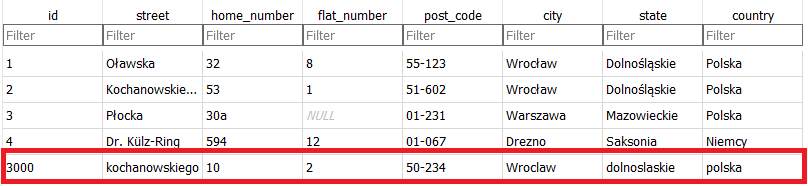
\includegraphics[width=1\linewidth]{images/image12.png}
	\caption{Wynik operacji wstawiania}
	\label{image12}
\end{figure}
	
	\item edycja rekordów w tabeli
	
\begin{figure}[h]
	\centering
	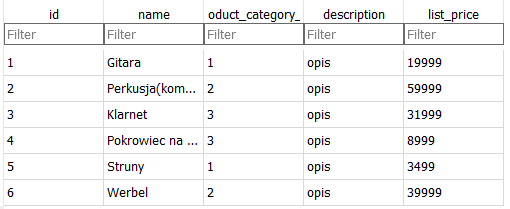
\includegraphics[width=0.6\linewidth]{images/image13.png}
	\caption{Tabela przed edycją}
	\label{image13}
\end{figure}
	
\begin{lstlisting}[style=SQLite]
UPDATE products SET description = 'Promocja'
WHERE list_price < 9000;
\end{lstlisting}
	
\newpage
\begin{figure}[h]
	\centering
	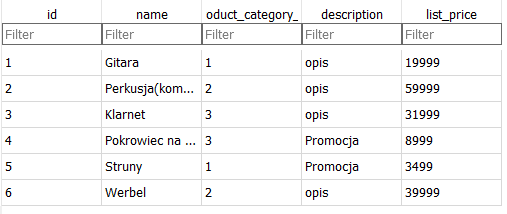
\includegraphics[width=0.6\linewidth]{images/image14.png}
	\caption{Tabela po edycji}
	\label{image14}
\end{figure}

	\item usuwanie rekordów
	
\begin{figure}[h]
	\centering
	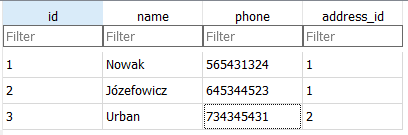
\includegraphics[width=0.6\linewidth]{images/image15.png}
	\caption{Tabela przed edycją}
	\label{image15}
\end{figure}

\begin{lstlisting}[style=SQLite]
DELETE FROM clients WHERE name = 'Nowak';
\end{lstlisting}

\begin{figure}[h]
	\centering
	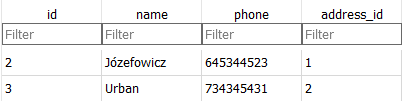
\includegraphics[width=0.5\linewidth]{images/image16.png}
	\caption{Tabela po edycji}
	\label{image16}
\end{figure}	
	
\end{itemize}

%%%%%%%%%%%%%%%%%%%%%%%%%%%%%%%%%%%%%%%%%%%%%%%%%%%%%%%%%%%%%%%%
\section{Implementacja i testy aplikacji}
%%%%%%%%%%%%%%%%%%%%%%%%%%%%%%%%%%%%%%%%%%%%%%%%%%%%%%%%%%%%%%%%
%%%%%%%%%%%%%%%%%%%%%%%%%%%%%%%%%%%%%%%%%%%%%%%%
\subsection{Instalacja i konfigurowanie systemu}
%%%%%%%%%%%%%%%%%%%%%%%%%%%%%%%%%%%%%%%%%%%%%%%%

Na chwilę obecną, oprogramowanie dostarczamy w postaci kodu źródłowego oraz pliku z~bazą danych. Niestety na chwilę obecną nie byliśmy w stanie wygenerować gotowych plików binarnych, które można byłoby uruchomić przy użyciu maszyny wirtualnej Javy.

Program można bez problemu uruchomić korzystając z dowolnego środowiska programistycznego do Javy (na przykład IntelliJ IDEA).

%%%%%%%%%%%%%%%%%%%%%%%%%%%%%%%%%%%%%%%%%%%%%%%%
\subsection{Instrukcja użytkowania aplikacji}
%%%%%%%%%%%%%%%%%%%%%%%%%%%%%%%%%%%%%%%%%%%%%%%%

Po uruchomieniu aplikacji, przywita nas widok, jak na rysunku \ref{image7}.

\begin{figure}[h]
	\centering
	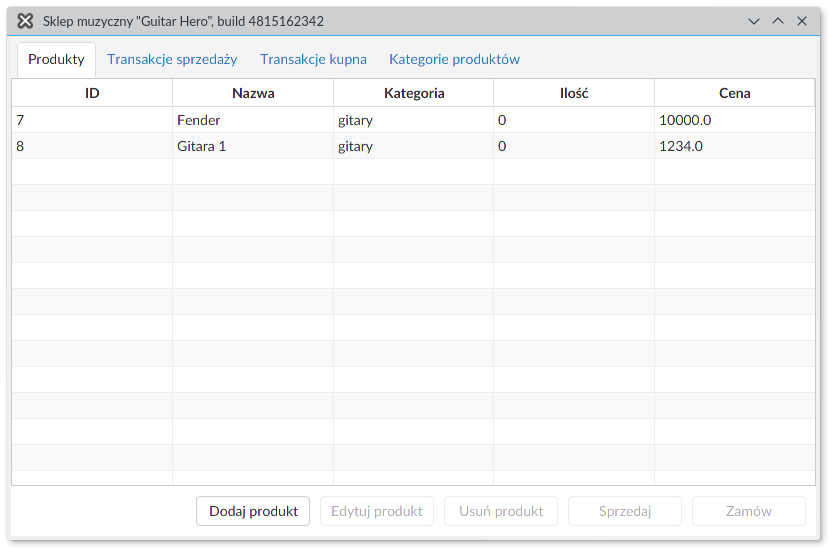
\includegraphics[width=0.7\linewidth]{images/image7.png}
	\caption{Domyślny widok aplikacji}
	\label{image7}
\end{figure}

Z tego miejsca możemy zobaczyć, jakie produkty są w naszej bazie oraz wykonywać na~nich podstawowe operacji dodawania, edycji oraz usuwania.

Możemy przenieść się do innej zakładki, gdzie możemy podejrzeć transakcje sprzedaży i~zakupu (zamówienia towaru przez sklep) oraz przenieść się do edycji kategorii produktów.

Aplikacja wydaje się być bardzo intuicyjna w użytkowaniu.


%%%%%%%%%%%%%%%%%%%%%%%%%%%%%%%%%%%%%%%%%%%%%%%%
\subsection{Testowanie opracowanych funkcji systemu}
%%%%%%%%%%%%%%%%%%%%%%%%%%%%%%%%%%%%%%%%%%%%%%%%

Przeprowadźmy test poprawności działania aplikacji na przykładzie edycji przykładowego produktu.

Rysunek \ref{image8} przedstawia stan aplikacji przed rozpoczęciem testu.

\newpage
\begin{figure}[h]
	\centering
	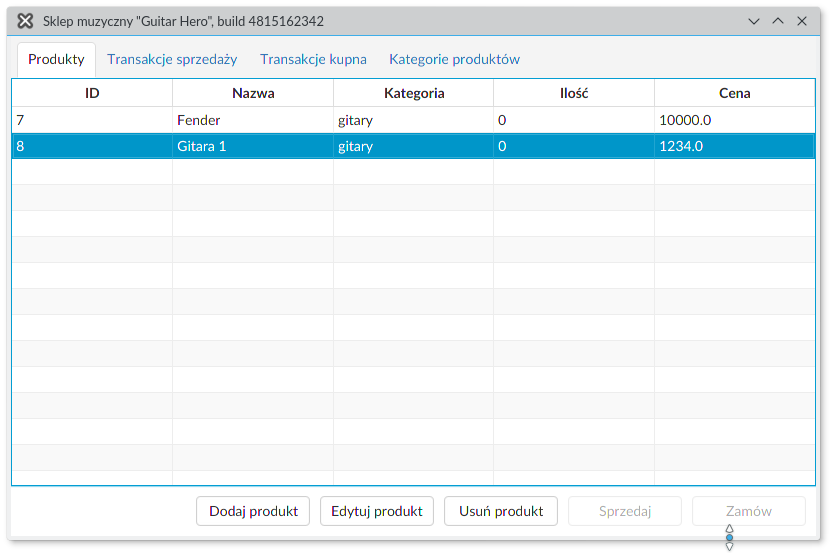
\includegraphics[width=0.6\linewidth]{images/image8.png}
	\caption{Zaznaczony element tabeli}
	\label{image8}
\end{figure}

Następnie naciskamy 'Dodaj produkt' i tym samym przechodzimy do edycji produktu. Efekt możemy zobaczyć na rysunku \ref{image9}.

\begin{figure}[h]
	\centering
	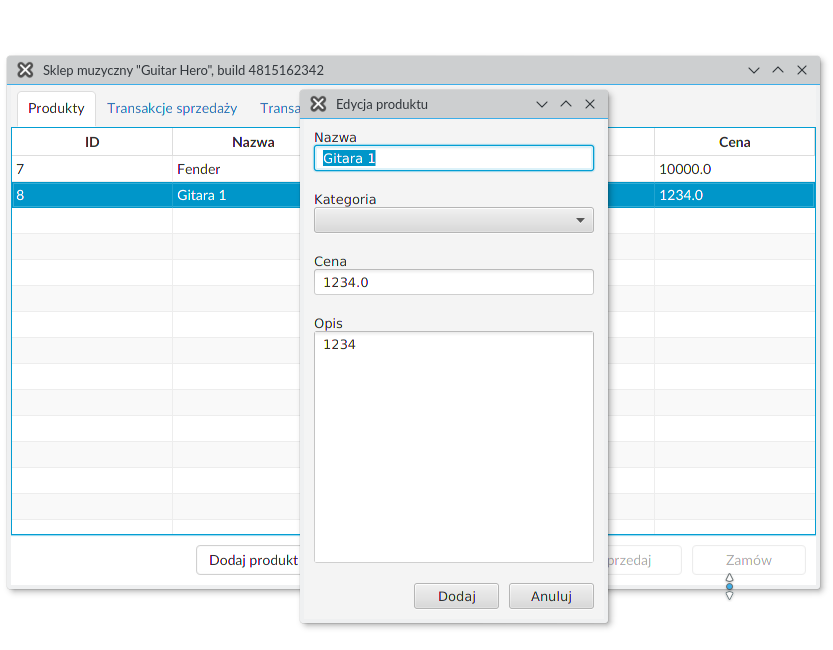
\includegraphics[width=0.5\linewidth]{images/image9.png}
	\caption{Okno edycji produktu}
	\label{image9}
\end{figure}

Modyfikujemy dane w polu 'Nazwa' na \emph{Gitara2} i sprawdzamy jaki będzie efekt. Po kliknięciu na 'Dodaj' program powróci do poprzedniego widoku. Rysunek \ref{image10} przedstawia efekt modyfikacji.

\newpage
\begin{figure}[h]
	\centering
	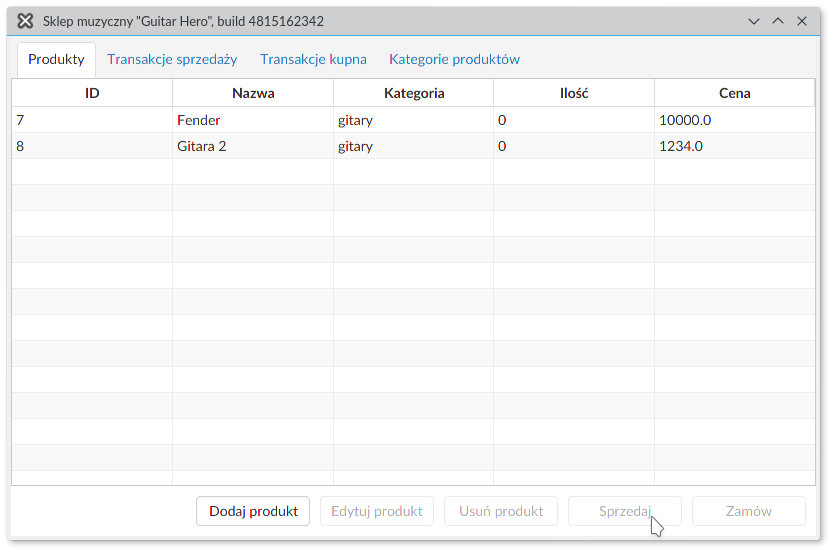
\includegraphics[width=0.7\linewidth]{images/image10.png}
	\caption{Zmodyfikowane dane}
	\label{image10}
\end{figure}

Podobne testy zostały wykonane dla pozostałych funkcjonalności aplikacji tj. dodawania i usuwania produktów oraz dodawania, modyfikacji i usuwania kategorii produktów.

%%%%%%%%%%%%%%%%%%%%%%%%%%%%%%%%%%%%%%%%%%%%%%%%
\subsection{Omówienie wybranych rozwiązań programistycznych}
%%%%%%%%%%%%%%%%%%%%%%%%%%%%%%%%%%%%%%%%%%%%%%%%
%%%%%%%%%%%%%%%%%%%%%%%%%%%%%%%%
\subsubsection{Implementacja interfejsu dostępu do bazy danych}
%%%%%%%%%%%%%%%%%%%%%%%%%%%%%%%%

W celu dostępu do bazy danych wykorzystaliśmy sterownik JDBC w Javie. Umożliwia on komunikację z bazą danych przy użyciu zapytań SQL. Dane są zwracane w postaci obiektów \lstinline|ResultSet|, które można następnie odczytać.

Dla każdej tabeli w bazie, zaimplementowaliśmy jej odpowiednik jako model danych w~Javie. Dla przykładu, tak prezentuje się klasa \emph{ItemCondition}, która reprezentuje jeden wiersz tabeli \lstinline|item_conditions|:

\begin{lstlisting}[style=Java]
public class ItemCondition implements TableRow {
	private final int id;
	private final String name;

	public ItemCondition(int id, String name) {
		this.id = id;
		this.name = name;
	}

	@Override
	public int getId() {
		return id;
	}

	public String getName() {
		return name;
	}

	@Override
	public PreparedStatement prepareInsertStatement(Connection connection, String sql) throws SQLException {
		PreparedStatement preparedStatement = connection.prepareStatement(sql);
		preparedStatement.setString(1, name);
		return preparedStatement;
	}

	@Override
	public PreparedStatement prepareUpdateStatement(Connection connection, String sql) throws SQLException {
		PreparedStatement preparedStatement = connection.prepareStatement(sql);
		preparedStatement.setString(1, name);
		preparedStatement.setInt(2, id);
		return preparedStatement;
	}
}
\end{lstlisting}

Jak można zauważyć, klasa ta nadpisuje pewne metody z interfejsu \emph{TableRow}. Interfejs \emph{TableRow} ma za zadanie ułatwić komunikację z bazą danych, udostępniając możliwość utworzenia tzw. \emph{statements}, które są wykorzystywane przy dodawaniu wierszy do tabeli, bądź edycji tych wierszy.

Interfejs ten posiada zdefiniowane domyślne metody, które nie muszą być nadpisywane przez klasy implementujące. Tak prezentuje się klasa \emph{TableRow}, wraz ze wspomnianymi metodami:

\begin{lstlisting}[style=Java]
public interface TableRow {
	public int getId();

	public default void insertInto(Database database, String sql) throws SQLException {
		prepareInsertStatement(database.connection(), sql)
			.executeUpdate();
	}

	public default void updateIn(Database database, String sql) throws SQLException {
		prepareUpdateStatement(database.connection(), sql)
			.executeUpdate();
	}

	public default void deleteFrom(Database database, String sql) throws SQLException {
		prepareDeleteStatement(database.connection(), sql)
			.executeUpdate();
	}

	public PreparedStatement prepareInsertStatement(Connection connection, String sql) throws SQLException;

	public PreparedStatement prepareUpdateStatement(Connection connection, String sql) throws SQLException;

	public default PreparedStatement prepareDeleteStatement(Connection connection, String sql) throws SQLException {
		PreparedStatement preparedStatement = connection.prepareStatement(sql);
		preparedStatement.setInt(1, getId());
		return preparedStatement;
	}
}
\end{lstlisting}

Domyślnie zostały zdefiniowane 4 metody, które nie różnią się wcale w zależności od tabeli, więc zrezygnowano z ich nadpisania w klasach implementujących interfejs. 3 metody są~odpowiedzialne za wstawianie, modyfikację oraz usuwanie danych z tabeli. Czwarta metoda jest podobna do tych wspomnianych wcześniej w klasie \emph{ItemCondition}. Służy do przygotowania tzw. \emph{statement} dla usuwania wiersza z tabeli. Metoda ta również jest identyczna dla wszystkich klas implementujących interfejs.

Podobnie jak pojedyncze wiersze, zostały reprezentowane całe tabele. Zdecydowano się stworzyć szereg klas, które będą umożliwiać pobranie całych tabel. W celu ułatwienia zadania, dodano interfejs \emph{Table}, który reprezentje tabelę:

\begin{lstlisting}[style=Java]
public interface Table {
	public default ArrayList<? extends TableRow> selectFrom(Database database, String sql) throws SQLException {
		Statement statement  = database.connection().createStatement();
		ArrayList<? extends TableRow> table = toList(database, statement.executeQuery(sql));
		return table;
	}

	public ArrayList<? extends TableRow> toList(Database database, ResultSet r) throws SQLException;

	public default int count(Database database, String sql, int id) throws SQLException {
		Statement statement  = database.connection().createStatement();
		ResultSet resultSet = statement.executeQuery(sql);
		return resultSet.getInt(1);
	}
}
\end{lstlisting}

Najważniejszym elementem jest tutaj metoda \lstinline|selectFrom|, która zwraca kolekcję zawierającą elementy dziedziczące po \emph{TableRow}. Umożliwia to szybkie "wybranie" calej tabeli i~osadzenie jej w kolekcji.

Kolejnym elementem implementacji bazy danych jest klasa \emph{Database}, która odpowiada za nawiązanie połaczenia z bazą danych. Obiekt tej klasy jest przekazywany do wszystkich operacji, które wykonujemy w bazie.

\begin{lstlisting}[style=Java]
public class Database {
	Connection connection;

	public Database(String connectionString) throws SQLException {
		connection = DriverManager.getConnection(connectionString);
	}

	public Connection connection() {
		return connection;
	}

	public void closeConnection() throws SQLException {
		connection.close();
	}
}
\end{lstlisting}

Tworząc obiekt typu \emph{Database} od razu nawiązujemy połączenie z bazą, którą podajemy przy użyciu \lstinline|connectionString|.

%%%%%%%%%%%%%%%%%%%%%%%%%%%%%%%%
\subsubsection{Implementacja wybranych funkcjonalności systemu}
%%%%%%%%%%%%%%%%%%%%%%%%%%%%%%%%

Dodawanie nowych produktów do bazy danych zostało zrealizowane w następujący sposób.

W JavaFX, aby wywołać akcję przy użyciu elementów interfejsu, należy zdefiniować kontroler. Zdefiniowaliśmy taki kontroler o nazwie \emph{ProductsController} dla widoku, gdzie znajduje się nasza tabela z produktami. W tym miejscu znalazła się metoda, która uruchamia się po~naciśnięciu przycisku:

\begin{lstlisting}[style=Java]
@FXML
private void handleNewProduct() {
	main.showAddProductDialog(null, "Dodawanie produktu");
}
\end{lstlisting}

Metoda wywołuje metodę \lstinline[style=Java]|showAddProductDialog(ProductView, String)| w klasie \emph{Main}. Metoda ta odpowiada za wywołanie nowego okna, które umożliwia dodanie nowego produktu. Dla nowo stworzonego okna także zdefiniowano kontroler, który wywołuje odpowiednią metodę po~naciśnięciu przycisku 'Dodaj':

\begin{lstlisting}[style=Java]
@FXML
private void handleAdd() {
	if (isInputValid()) {
		int id = 0;
		if (productView != null) {
			id = Integer.parseInt(productView.getId());
		}
		Product product = new Product.Builder(id)
			.name(nameTextField.getText())
			.productCategoryId(productCategoryComboBox.getValue().getId())
			.description(descriptionTextArea.getText())
			.price((int) Float.parseFloat(priceTextField.getText()) * 100)
			.build();
		stage.close();
		if (productView != null) {
			try {
				product.updateIn(main.data().database(), "UPDATE products SET name = ?, product_category_id = ?, description = ?, price = ? WHERE id = ?");
			} catch (SQLException e) {
				e.printStackTrace();
			}
		} else {
			try {
				product.insertInto(main.data().database(), "INSERT INTO products(name, product_category_id, description, price) values(?, ?, ?, ?)");
			} catch (SQLException e) {
				e.printStackTrace();
			}
		}
		overviewController.productsController().update();
	}
}
\end{lstlisting}

Metoda, na początku sprawdza czy wprowadziliśmy odpowiednie dane w polach. Następnie sprawdzamy czy produkt (\emph{ProductView}), już istnieje (będzie edytowany) czy nie istnieje, i~należy go utworzyć.

W następnym kroku tworzymy nowy obiekt na podstawie pobranych danych z formularzy. Zamykamy okno i dodajemy produkt do bazy, bądź go modyfikujemy.

W ostatnim kroku, wywołujemy funkcję update na kontrolerze z produktami, w celu zaktualizowania widoku tabeli.

%%%%%%%%%%%%%%%%%%%%%%%%%%%%%%%%
\subsubsection{Implementacja mechanizmów bezpieczeństwa}
%%%%%%%%%%%%%%%%%%%%%%%%%%%%%%%%

Z powodu braku zabezpieczeń bazy SQLite zdecydowaliśmy się stworzyć system logowania dla użytkowników aplikacji. Niestety funkcjonalności nie udało nam się w porę zaimplementować.

%%%%%%%%%%%%%%%%%%%%%%%%%%%%%%%%%%%%%%%%%%%%%%%%%%%%%%%%%%%%%%%%
\section{Podsumowanie i wnioski}
%%%%%%%%%%%%%%%%%%%%%%%%%%%%%%%%%%%%%%%%%%%%%%%%%%%%%%%%%%%%%%%%

Realizacja projektu pozwoliła na zdobycie cennych umięjętności pracy z bazami danych. Mogliśmy poznać nowe, nieznane dotychczas technologie i wykorzystać je przy pisaniu aplikacji, która byłaby w stanie funkcjonować w prawdziwych warunkach produkcyjnych.

Brak czasu w trakcie realizacji projektu sprawił, że nie udało się zaimplementować wszystkich funkcjonalności, które chcielibyśmy w takiej aplikacji widzieć.

Ponadto, nie wszystkie decyzje projektowe ostatecznie okazały się trafionymi pomysłami. W celu integracji bazy danych z aplikacją mogliśmy wykorzystać system \emph{ORM} (jak na przykład Hibernate), który oszczędził by sporo pracy przy pisaniu kodu pobierającego dane z bazy danych.

Nietrafionym pomysłem było również wykorzystanie bazy danych SQLite. Brak wsparcia dla zarządzania użytkownikami oraz mechanizmów zabezpieczeń powoduje spore utrudnienia w utrzymaniu i zabezpieczeniu systemu.

Błędem projektowym okazał się również brak dodatkowych mechanizmów w bazie (na przykład triggerów), które ułatwiłyby zarządzanie danymi na poziomie kodu źródłowego aplikacji. Ponadto mogliśmy wykorzystać więcej widoków, w celu ułatwienia dostępu do bazy i~zapewnienia lepszych możliwości rozbudowy systemu na przyszłość.

Trudnością w czasie realizacji aplikacji dostępowej okazała się JavaFX, która znacznie spowolniła pracę, głównie przez nasz brak umiejętności w zakresie budowania aplikacji z interfejsem graficznym.

Podsumowując. Projekt okazał się dość ciężki w realizacji, co jednak zaowocowało lepszym zrozumieniem tematu i daniem możliwości unikania podobnych błędów na przyszłość.

\end{document}